\documentclass[dvipdfmx]{jarticle}
\usepackage{graphicx}
\usepackage{tikz}
\usetikzlibrary{calc}
\pagestyle{empty}
%\newcommand{\cstatline}[2]{\node[anchor=west] at (${#1}*(0,-0.5)$) {\texttt{#2}};}
\begin{document}
 \begin{tabular}{ccc}
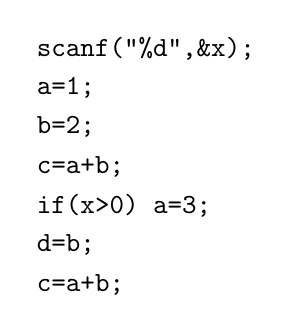
\begin{tikzpicture}
   \node[anchor=west] at ($0*(0,-0.5)$) {\texttt{scanf("\%d",\&x);}};
   \node[anchor=west] at ($1*(0,-0.5)$) {\texttt{a=1;}};
   \node[anchor=west] at ($2*(0,-0.5)$) {\texttt{b=2;}};
   \node[anchor=west] at ($3*(0,-0.5)$) {\texttt{c=a+b;}};
   \node[anchor=west] at ($4*(0,-0.5)$) {\texttt{if(x>0) a=3;}};
   \node[anchor=west] at ($5*(0,-0.5)$) {\texttt{d=b;}};
   \node[anchor=west] at ($6*(0,-0.5)$) {\texttt{c=a+b;}};
\end{tikzpicture}
  & $\Rightarrow$ &
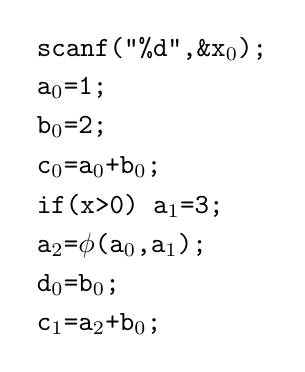
\begin{tikzpicture}
   \node[anchor=west] at ($0*(0,-0.5)$) {\texttt{scanf("\%d",\&x$_0$);}};
   \node[anchor=west] at ($1*(0,-0.5)$) {\texttt{a$_0$=1;}};
   \node[anchor=west] at ($2*(0,-0.5)$) {\texttt{b$_0$=2;}};
   \node[anchor=west] at ($3*(0,-0.5)$) {\texttt{c$_0$=a$_0$+b$_0$;}};
   \node[anchor=west] at ($4*(0,-0.5)$) {\texttt{if(x>0) a$_1$=3;}};
   \node[anchor=west] at ($5*(0,-0.5)$) {\texttt{a$_2$=$\phi$(a$_0$,a$_1$);}};
   \node[anchor=west] at ($6*(0,-0.5)$) {\texttt{d$_0$=b$_0$;}};
   \node[anchor=west] at ($7*(0,-0.5)$) {\texttt{c$_1$=a$_2$+b$_0$;}};
\end{tikzpicture}
 \end{tabular}
\end{document}
